% Captioned music model (450M, F1 layout), drawn in the style of Sebastian Raschka's LLM architecture gallery:
% main column in a grey container, the repeated block in teal with dashed sublayers, zoom panels with dotted borders,
% the anti-forgetting training recipe as a panel and a monospace list. Shapes from musicar/model/gpt.py, recipe from
% config/pilots/section_*.py + train.py, switch shares from logs/sections/forget.md.
% Build: pdflatex architecture.tex  (TinyTeX: export PATH=$HOME/.local/bin:$PATH)
% SVG / PNG: pdftocairo -svg architecture.pdf architecture.svg ; pdftocairo -png -r 200 -singlefile architecture.pdf architecture
\documentclass[border=8pt]{standalone}
\usepackage[scaled=0.92]{helvet}
\renewcommand{\familydefault}{\sfdefault}
\usepackage{inconsolata}
\usepackage{amsmath}
\usepackage{tikz}
\usetikzlibrary{arrows.meta,calc,decorations.pathreplacing,backgrounds}

\definecolor{tealT}{HTML}{3B7D70}   % title, brace
\definecolor{tealF}{HTML}{C3E0D6}   % repeated block
\definecolor{tealB}{HTML}{6FA696}
\definecolor{greyF}{HTML}{E4E4E4}   % model container
\definecolor{greyB}{HTML}{9C9C9C}
\definecolor{pinkL}{HTML}{C2577A}   % caption path: lines, labels
\definecolor{pinkF}{HTML}{F6CCD9}
\definecolor{boxG}{HTML}{D5D5D5}    % plain linear layers in zooms
\definecolor{dark}{HTML}{4A4A4A}    % the component a zoom opens
\definecolor{blueF}{HTML}{CFE0F2}   % the second file in a spliced window

\tikzset{
  box/.style={draw=black, fill=white, rounded corners=3pt, minimum height=5.6mm, inner sep=3pt, align=center,
              font=\footnotesize, line width=0.6pt},
  gbox/.style={box, fill=boxG},
  pbox/.style={box, fill=pinkF, draw=pinkL},
  dbox/.style={box, fill=dark, draw=dark, text=white},
  sub/.style={draw=pinkL, dashed, rounded corners=6pt, line width=0.9pt},
  zoom/.style={draw=black, densely dotted, rounded corners=10pt, line width=1.5pt},
  arr/.style={-{Stealth[length=2.4mm]}, line width=0.9pt},
  parr/.style={arr, draw=pinkL},
  sum/.style={draw=black, fill=white, circle, inner sep=0pt, minimum size=4.6mm, line width=0.8pt},
  tok/.style={draw=black, minimum width=2.9mm, minimum height=2.9mm, inner sep=0pt, line width=0.4pt},
  plab/.style={text=pinkL, font=\footnotesize\bfseries},
  note/.style={font=\scriptsize, text=black!75, align=left},
  head/.style={box, minimum width=12mm, inner sep=2pt},
}

\begin{document}
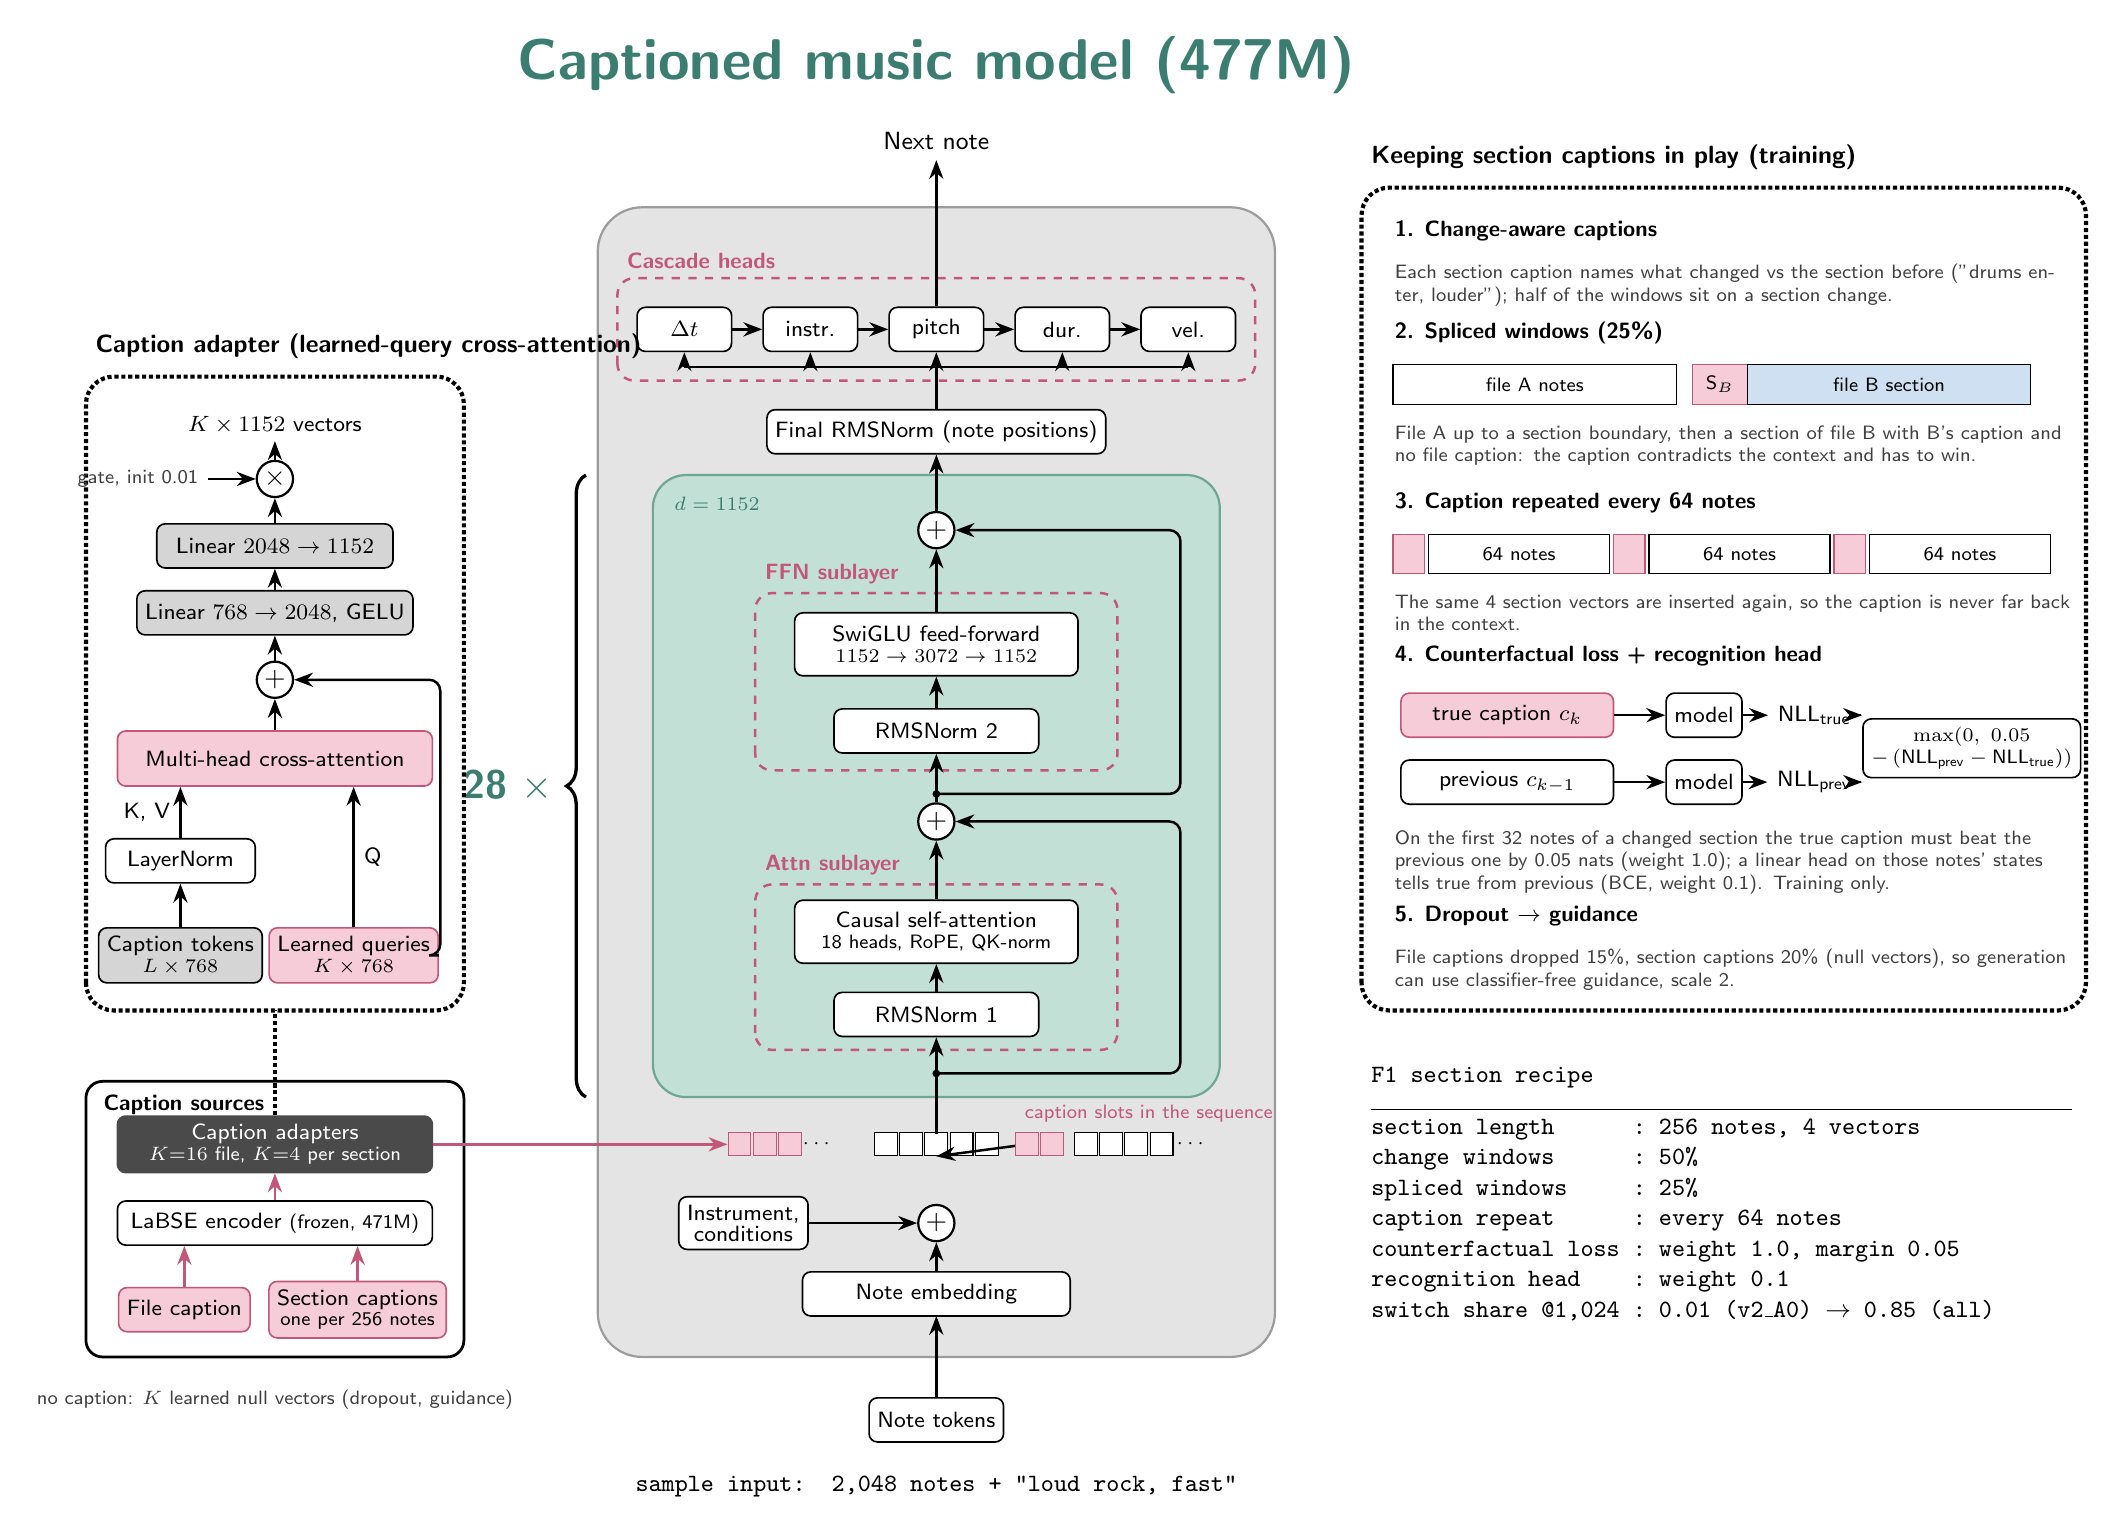
\begin{tikzpicture}

%% ================= main column =================
\node[font=\fontsize{20}{22}\selectfont\bfseries, text=tealT] at (0, 16.55) {Captioned music model (477M)};

% container
\begin{scope}[on background layer]
  \fill[greyF, draw=greyB, rounded corners=16pt, line width=0.8pt] (-4.3, 0.15) rectangle (4.3, 14.75);
  \fill[tealF, draw=tealB, rounded corners=12pt, line width=0.8pt] (-3.6, 3.45) rectangle (3.6, 11.35);
\end{scope}

% input
\node[box] (inp) at (0, -0.65) {Note tokens};
\node[font=\ttfamily\small] at (0, -1.5) {sample input: 2,048 notes + "loud rock, fast"};
\draw[arr] (inp) -- (0, 0.67);

% embedding + conditions
\node[box, minimum width=34mm] (emb) at (0, 0.95) {Note embedding};
\node[sum] (s0) at (0, 1.85) {$+$};
\node[box] (cond) at (-2.45, 1.85) {Instrument,\\[-2pt] conditions};
\draw[arr] (emb) -- (s0);
\draw[arr] (cond) -- (s0);

% interleaved sequence
\foreach \i in {0,1,2} { \node[tok, fill=pinkF, draw=pinkL] (p\i) at (-2.5+0.32*\i, 2.85) {}; }
\node[font=\scriptsize] at (-1.5, 2.85) {$\cdots$};
\foreach \i in {0,...,4} { \node[tok, fill=white] (n\i) at (-0.64+0.32*\i, 2.85) {}; }
\foreach \i in {0,1} { \node[tok, fill=pinkF, draw=pinkL] (s\i) at (1.15+0.32*\i, 2.85) {}; }
\foreach \i in {0,...,3} { \node[tok, fill=white] (m\i) at (1.9+0.32*\i, 2.85) {}; }
\node[font=\scriptsize] at (3.25, 2.85) {$\cdots$};
\draw[arr] (s0) -- (n2.south);
\node[text=pinkL, font=\scriptsize, anchor=south west, align=left] at (1.0, 3.0) {caption slots in the sequence};

% transformer block
\node[box, minimum width=26mm] (ln1) at (0, 4.5) {RMSNorm 1};
\node[box, minimum width=36mm, minimum height=8mm] (att) at (0, 5.55) {Causal self-attention\\[-2pt] {\scriptsize 18 heads, RoPE, QK-norm}};
\node[sum] (a1) at (0, 6.95) {$+$};
\node[box, minimum width=26mm] (ln2) at (0, 8.1) {RMSNorm 2};
\node[box, minimum width=36mm, minimum height=8mm] (ffn) at (0, 9.2) {SwiGLU feed-forward\\[-2pt] {\scriptsize $1152\to3072\to1152$}};
\node[sum] (a2) at (0, 10.65) {$+$};
\draw[sub] (-2.3, 4.05) rectangle (2.3, 6.15);
\node[plab, anchor=south west] at (-2.3, 6.15) {Attn sublayer};
\draw[sub] (-2.3, 7.6) rectangle (2.3, 9.85);
\node[plab, anchor=south west] at (-2.3, 9.85) {FFN sublayer};
\draw[arr] (0, 2.98) -- (ln1);
\draw[arr] (ln1) -- (att);
\draw[arr] (att) -- (a1);
\draw[arr] (a1) -- (ln2);
\draw[arr] (ln2) -- (ffn);
\draw[arr] (ffn) -- (a2);
\draw[arr, rounded corners=4pt] (0, 3.75) -- (3.1, 3.75) |- (a1.east);
\draw[arr, rounded corners=4pt] (0, 7.3) -- (3.1, 7.3) |- (a2.east);
\fill (0, 3.75) circle (1.4pt);
\fill (0, 7.3) circle (1.4pt);

% repeat brace
\draw[decorate, decoration={brace, amplitude=7pt}, line width=1.2pt, draw=black] (-4.45, 3.45) -- (-4.45, 11.35);
\node[font=\fontsize{15}{17}\selectfont\bfseries, text=tealT, anchor=east] at (-4.75, 7.4) {28 $\times$};
\node[note, anchor=north west, text=tealT] at (-3.45, 11.2) {$d = 1152$};

% final norm + cascade heads
\node[box, minimum width=34mm] (lnf) at (0, 11.9) {Final RMSNorm (note positions)};
\draw[arr] (a2) -- (lnf);
\draw[sub] (-4.05, 12.55) rectangle (4.05, 13.85);
\node[plab, anchor=south west] at (-4.05, 13.85) {Cascade heads};
\node[head] (h1) at (-3.2, 13.2) {$\Delta t$};
\node[head] (h2) at (-1.6, 13.2) {instr.};
\node[head] (h3) at (0, 13.2) {pitch};
\node[head] (h4) at (1.6, 13.2) {dur.};
\node[head] (h5) at (3.2, 13.2) {vel.};
\draw[line width=0.9pt] (lnf.north) -- (0, 12.72);
\draw[line width=0.9pt] (-3.2, 12.72) -- (3.2, 12.72);
\foreach \h in {h1,h2,h4,h5} { \draw[arr] (\h.south |- 0,12.72) -- (\h.south); }
\draw[arr] (0, 12.72) -- (h3.south);
\foreach \a/\b in {h1/h2,h2/h3,h3/h4,h4/h5} { \draw[arr] (\a.east) -- (\b.west); }
\draw[arr] (h3.north) -- (0, 15.35);
\node[font=\small] at (0, 15.6) {Next note};

%% ================= caption sources (left, bottom) =================
\draw[line width=1pt, rounded corners=6pt] (-10.8, 0.15) rectangle (-6.0, 3.65);
\node[font=\footnotesize\bfseries, anchor=north west] at (-10.7, 3.6) {Caption sources};
\node[pbox] (fc) at (-9.55, 0.75) {File caption};
\node[pbox] (sc) at (-7.35, 0.75) {Section captions\\[-2pt] {\scriptsize one per 256 notes}};
\node[box, minimum width=40mm] (lab) at (-8.4, 1.85) {LaBSE encoder {\scriptsize (frozen, 471M)}};
\node[dbox, minimum width=40mm] (ad) at (-8.4, 2.85) {Caption adapters\\[-2pt] {\scriptsize $K{=}16$ file, $K{=}4$ per section}};
\draw[parr] (fc) -- (fc |- lab.south);
\draw[parr] (sc) -- (sc |- lab.south);
\draw[parr] (lab) -- (ad);
\draw[parr, rounded corners=4pt] (ad.east) -- (-3.0, 2.85) -- (p0.west);
\node[note, anchor=north] at (-8.4, -0.15) {no caption: $K$ learned null vectors (dropout, guidance)};

%% ================= zoom: caption adapter (left, top) =================
\draw[zoom] (-10.8, 4.55) rectangle (-6.0, 12.6);
\node[font=\small\bfseries, anchor=south west] at (-10.8, 12.7) {Caption adapter (learned-query cross-attention)};
\draw[densely dotted, line width=1.5pt] (ad.north) -- (-8.4, 4.55);
\node[gbox, minimum width=19mm] (X) at (-9.6, 5.25) {Caption tokens\\[-2pt] {\scriptsize $L\times768$}};
\node[pbox, minimum width=19mm] (P) at (-7.4, 5.25) {Learned queries\\[-2pt] {\scriptsize $K\times768$}};
\node[box, minimum width=19mm] (lnx) at (-9.6, 6.45) {LayerNorm};
\node[pbox, minimum width=40mm, minimum height=7mm] (xa) at (-8.4, 7.75) {Multi-head cross-attention};
\node[sum] (b1) at (-8.4, 8.75) {$+$};
\node[gbox, minimum width=30mm] (l1) at (-8.4, 9.6) {Linear $768\to2048$, GELU};
\node[gbox, minimum width=30mm] (l2) at (-8.4, 10.45) {Linear $2048\to1152$};
\node[sum] (g) at (-8.4, 11.3) {$\times$};
\node[note, anchor=east] (gl) at (-9.25, 11.3) {gate, init 0.01};
\node[font=\footnotesize, anchor=south] at (-8.4, 11.75) {$K\times1152$ vectors};
\draw[arr] (X) -- (lnx);
\draw[arr] (lnx.north) -- node[left, font=\footnotesize] {K, V} (lnx.north |- xa.south);
\draw[arr] (P.north) -- node[right, font=\footnotesize] {Q} (P.north |- xa.south);
\draw[arr] (xa) -- (b1);
\draw[arr, rounded corners=4pt] (P.east) -- (-6.3, 5.25) |- (b1.east);
\draw[arr] (b1) -- (l1);
\draw[arr] (l1) -- (l2);
\draw[arr] (l2) -- (g);
\draw[arr] (gl.east) -- (g.west);
\draw[arr] (g) -- (-8.4, 11.78);

%% ================= zoom: anti-forgetting recipe (right) =================
\draw[zoom] (5.4, 4.55) rectangle (14.6, 15.0);
\node[font=\small\bfseries, anchor=south west] at (5.4, 15.1) {Keeping section captions in play (training)};

% 1 change-aware captions
\node[font=\footnotesize\bfseries, anchor=west] at (5.7, 14.45) {1. Change-aware captions};
\node[note, anchor=north west, text width=8.6cm] at (5.7, 14.15)
  {Each section caption names what changed vs the section before ("drums enter, louder"); half of the windows sit on a section change.};

% 2 splice windows
\node[font=\footnotesize\bfseries, anchor=west] at (5.7, 13.15) {2. Spliced windows (25\%)};
\node[draw=black, fill=white, minimum width=36mm, minimum height=5mm, font=\scriptsize] (sa) at (7.6, 12.5) {file A notes};
\node[draw=pinkL, fill=pinkF, minimum width=7mm, minimum height=5mm, font=\scriptsize] (sb) at (9.95, 12.5) {S$_B$};
\node[draw=black, fill=blueF, minimum width=36mm, minimum height=5mm, font=\scriptsize] (sbn) at (12.1, 12.5) {file B section};
\node[note, anchor=north west, text width=8.6cm] at (5.7, 12.1)
  {File A up to a section boundary, then a section of file B with B's caption and no file caption: the caption contradicts the context and has to win.};

% 3 repeat
\node[font=\footnotesize\bfseries, anchor=west] at (5.7, 11.0) {3. Caption repeated every 64 notes};
\foreach \i in {0,1,2} {
  \node[draw=pinkL, fill=pinkF, minimum width=4mm, minimum height=5mm, inner sep=0pt] at (6.0+2.8*\i, 10.35) {};
  \node[draw=black, fill=white, minimum width=23mm, minimum height=5mm, font=\scriptsize] at (7.4+2.8*\i, 10.35) {64 notes};
}
\node[note, anchor=north west, text width=8.6cm] at (5.7, 9.95)
  {The same 4 section vectors are inserted again, so the caption is never far back in the context.};

% 4 counterfactual loss
\node[font=\footnotesize\bfseries, anchor=west] at (5.7, 9.05) {4. Counterfactual loss + recognition head};
\node[pbox, minimum width=27mm] (ct) at (7.25, 8.3) {true caption $c_k$};
\node[box, minimum width=27mm] (cp) at (7.25, 7.45) {previous $c_{k-1}$};
\node[box] (mt) at (9.75, 8.3) {model};
\node[box] (mp) at (9.75, 7.45) {model};
\node[font=\footnotesize] (nt) at (11.15, 8.3) {NLL$_\text{true}$};
\node[font=\footnotesize] (np) at (11.15, 7.45) {NLL$_\text{prev}$};
\draw[arr] (ct) -- (mt); \draw[arr] (cp) -- (mp);
\draw[arr] (mt) -- (nt); \draw[arr] (mp) -- (np);
\node[box, align=center, font=\scriptsize] (hinge) at (13.15, 7.88) {$\max(0,\ 0.05$\\$-\,(\text{NLL}_\text{prev}-\text{NLL}_\text{true}))$};
\draw[arr] (nt.east) -- (hinge.west |- nt.east);
\draw[arr] (np.east) -- (hinge.west |- np.east);
\node[note, anchor=north west, text width=8.6cm] at (5.7, 6.95)
  {On the first 32 notes of a changed section the true caption must beat the previous one by 0.05 nats (weight 1.0); a linear head on those notes' states tells true from previous (BCE, weight 0.1). Training only.};

% 5 guidance
\node[font=\footnotesize\bfseries, anchor=west] at (5.7, 5.75) {5. Dropout $\to$ guidance};
\node[note, anchor=north west, text width=8.6cm] at (5.7, 5.45)
  {File captions dropped 15\%, section captions 20\% (null vectors), so generation can use classifier-free guidance, scale 2.};

%% ================= recipe list (right, bottom) =================
\node[font=\ttfamily\small, anchor=north west, align=left] at (5.4, 3.95) {%
\textbf{F1 section recipe}\\[-1pt]
\rule{8.9cm}{0.6pt}\\
\begin{tabular}{@{}l@{\ :\ }l@{}}
section length      & 256 notes, 4 vectors\\
change windows      & 50\%\\
spliced windows     & 25\%\\
caption repeat      & every 64 notes\\
counterfactual loss & weight 1.0, margin 0.05\\
recognition head    & weight 0.1\\
switch share @1,024 & 0.01 (v2\_A0) $\to$ 0.85 (all)\\
\end{tabular}};

\end{tikzpicture}
\end{document}
